\documentclass[a4paper,11pt]{article}
 
% --- Packages
\usepackage{booktabs}
\usepackage[margin=1.5cm]{caption}
\usepackage{float}
\usepackage[table,xcdraw]{xcolor}
\usepackage{graphicx}
\usepackage{amsfonts,amsthm,amsmath,mathtools,graphicx,geometry}
\usepackage{enumitem} 
\usepackage{multicol}
\DeclareMathOperator*{\argmin}{arg\,min}

% --- Custom commands
\newcommand{\norm}[1]{\left\lVert#1\right\rVert}
\newcommand{\red}[1]{\textcolor{red}{#1}}
%% define command for averaging operator
\newcommand{\chevron}[1]{\left\langle #1 \right\rangle}
\newcommand{\pderiv}[3][]{% \pderiv[<order>]{<func>}{<var>} 
  \ensuremath{\frac{\partial^{#1} {#2}}{\partial {#3}^{#1}}}}
\newcommand{\noi}{\noindent}
\newcommand{\ep}{\epsilon} 
\newcommand{\pr}{\partial}
% --- Formatting 
\geometry{margin=1in}
\title{\vspace{-4ex}RANS Modeling in a Channel}
\author{Gopal Yalla, Clark Pederson, Tim Smith, Sean Carney}
\date{\today}

\pdfinfo{%
  /Title    (RANS Modeling in a Channel)
  /Author   (Gopal Yalla, Clark Pederson, Tim Smith, Sean Carney)
}
\graphicspath{ {figs/} }
\DeclareGraphicsExtensions{{.png,.pdf}}

\begin{document}
\maketitle
\section{Developing the channel flow equations}

We begin by developing the $k-\epsilon$ model for channel flow with Durbin's
$\overline{v^2}-f$ formulation of the eddy viscosity near
the wall. We chose this wall treatment since it fundamentally addresses the fact that near
the wall, the eddy viscosity transports momentum in the verticle direction, and
thus it should be a function of the wall normal velocity fluctuations.

Although we are ultimately interested in fully developed channel flow, so that averaged quantities that are independent of time, we choose not to discretize the steady Reynolds averaged Navier-Stokes equations for computational reasons. As is well known, the convergence of nonlinear solvers for discrete systems of nonlinear equations (e.g. Newton's method) requires the initial guess be in a neighborhood of the solution. Hence, unless a very accurate initial guess is provided, a nonlinear solver for the $\overline{v^2}-f$ model will diverge. To circumvent this issue, we choose to evolve our initial guess forward in time until a steady state is reached. This procedure is detailed in section 1.3. 

We thus consider the unsteady incompressible Reynolds averaged Navier-Stokes equations, 
$k-\epsilon$, and $\overline{v^2}-f$ model equations, which are given as:

\begin{align}
\pderiv{U_i}{x_i} &= 0 \label{eq:continuity} \\
\pderiv{U_i}{t} + U_j\pderiv{U_i}{x_j} &= -\pderiv{P}{x_i} +
\pderiv{}{x_j}\left(\nu\pderiv{U_i}{x_j} - r_{ij}\right) \\
\pderiv{k}{t} + U_j\pderiv{k}{x_j} &= -r_{ij}\pderiv{U_i}{x_j} - \epsilon +
\pderiv{}{x_j}\left(\frac{\nu_T}{\sigma_k}\pderiv{k}{x_j}\right) +
\nu\frac{\partial^2 k}{\partial x_j \partial x_j} \\
\pderiv{\epsilon}{t} + U_j\pderiv{\epsilon}{x_j} &=
-\frac{1}{T}\left(C_{\epsilon 1} \mathcal{P} + C_{\epsilon 2} \epsilon\right) +
\pderiv{}{x_j}\left(\frac{\nu_T}{\sigma_\epsilon}\pderiv{\epsilon}{x_j}\right) +
\nu\frac{\partial^2 \epsilon}{\partial x_j \partial x_j} \\
\pderiv{\overline{v^2}}{t} + U_j\pderiv{\overline{v^2}}{x_j} &= kf +
\pderiv{}{x_j}\left((\nu_T+\nu)\pderiv{\overline{v^2}}{x_j}\right) - \epsilon
\frac{\overline{v^2}}{k} \\
0 &=  f -  L^2 \nabla^2 f  -C_2 \frac{\mathcal{P}}{k} + \frac{C_1}{T} \left(
\frac{\overline{v^2}}{k} - \frac{2}{3} \right) 
%r_{ij} &= -\nu_T \left(\pderiv{U_i}{x_j} + \pderiv{U_j}{x_i}\right) + \frac{2
%k}{3}\delta_{ij} \\ 
%\nu_T &= \frac{3}{2}C_\mu\overline{v^2}T 
\label{eq:redistribution}
\end{align}

\noi where 

\begin{align*}
r_{ij} &= -\nu_T\left(\pderiv{U_i}{x_j} + \pderiv{U_j}{x_i}\right) +
\frac{2k}{3}\delta_{ij}\\
\nu_T &= \frac{3}{2}C_\mu \overline{v^2} T \\
\mathcal{P} &= \nu_T\left( \pderiv{U_j}{x_i} + \pderiv{U_i}{x_j}\right)\pderiv{U_j}{x_i} \\
T &= \max \left\{ \frac{k}{\ep} , 6 \left( \frac{\nu}{\ep} \right)^{\frac{1}{2}}
\right\} \\
L &= \max \left\{ C_L \frac{k^{3/2}}{\ep}, C_\eta \left( \frac{\nu^3}{\ep}
\right)^{1/4} \right\}
\end{align*}

We consider channel flow through a rectangular duct of height $h= 2\delta$, with
the bottom and top walls at $y=0$ and $y=2\delta$, and the midplane at
$y=\delta$.
Here we are modeling ``fully developed'' channel flow in the streamwise, $x$,
direction such that statistics do not change in the spanwise, $z$, or
streamwise directions. As in Pope \cite{pope} we neglect the mean spanwise
velocity. 
We enforce the no slip condition at the boundary, so that
$U_i=u_i=0 \, \forall i$. Since at the wall
$\pderiv{U}{x}=\pderiv{W}{z} = 0$, continuity implies that
$\pderiv{V}{y}=0$ and thus $V=0$ everywhere. Moreover, the flow is statistically
symmetric about the mid-plane $y = \delta$. These assumptions and conditions
imply that the original system, Eqns.
(\ref{eq:continuity})-(\ref{eq:redistribution}), is simplified to: 

\begin{align}
	\label{eq:ssv2f1}
        \pderiv{U}{t} &= -\pderiv{P}{x} +
\pderiv{}{y}\left((\nu+\nu_T)\pderiv{U}{y}\right) \\
        \pderiv{k}{t} &= \nu_T\left(\pderiv{U}{y}\right)^2 + 
\pderiv{}{y}\left((\nu+\frac{\nu_T}{\sigma_k})\pderiv{k}{y}\right) \\
        \pderiv{\ep}{t} &= \frac{1}{T}\left(C_{\ep
1}\nu_T\left(\pderiv{U}{y}\right)^2 - C_{\ep 2}\ep\right) + 
\pderiv{}{y}\left((\nu+\frac{\nu_T}{\sigma_\ep})\pderiv{\ep}{y}\right) \\
        \pderiv{\overline{v^2}}{t} &= kf - \frac{1}{T}\overline{v^2} +
\pderiv{}{y}\left((\nu+\nu_T)\pderiv{\overline{v}}{y}\right) \\
        0 &= \left( L^2\frac{\partial^2}{\partial y^2} - I\right)f +
C_2\frac{\nu_T}{k}\left(\pderiv{U}{y}\right)^2 -
\frac{C_1}{T}\left(\frac{\overline{v^2}}{k}-\frac{2}{3}\right)
	\label{eq:ssv2f5}
\end{align}

The constants are defined as follows: 
\begin{multicols}{2}
\begin{enumerate}
	\item $C_\mu = 0.09$
        \item $C_k = 1.0$
	\item $\sigma_\ep = 1.3$
	\item $C_2 = 0.4$	
\end{enumerate}
\columnbreak 

\begin{itemize}
	\item[5.] $C_1 = 0.3$
	\item[6.] $C_{\ep 1} = 1.4[1 + 0.045 \sqrt{k/\overline{v^2}}]$
	\item[7.] $C_{\ep 2} = 1.92$  
	\item[8.] $C_\eta = 16$
	\item[9.] $C_L = 0.2$
\end{itemize}
\end{multicols}

\subsection{Boundary conditions}
For the turbulent channel, we only compute for $y \in [0,\delta] $, as oppposed to the full $y \in [0,2\delta]$, by symmetry. The boundary conditions for our five dependent variables, $U, k, \ep, \overline{v^2}, f$, are as follows: 
\[
U = k = \overline{v^2} = 0 
\]
at $y = 0$, which comes from the no-slip condition, which then implies 
\[
\epsilon \to 2\nu \frac{k}{y^2}, \,\,\,\,\,\,\, f \to -\frac{20 \nu^2 \overline{v^2} }{\ep(0) y^4}
\]
at $y = 0$. As a consequence of symmetry, we require homogeneous Neumann conditions on all of the dependent variables: 
\[
\pderiv{U}{y}= \pderiv{\ep}{y} = \pderiv{\overline{v^2}}{y} = \pderiv{k}{y} = \pderiv{f}{y} = 0
\] 

\subsection{Nondimensionalization of the governing equations}
Here we nondimensionalize \eqref{eq:ssv2f1}-\eqref{eq:ssv2f5} using the characteristic velocity scale $u_{\tau}$ (the friction velocity) and length scale $\delta$. We then make the following nondimensionalizations:

\begin{multicols}{2}
\begin{enumerate}
\item $U^+ = U\big/u_{\tau}$
\item $\eta  = y\Big/\delta$
\item $t^+ = t\Big/(\delta/u_{\tau}), \,\,\,\, T^+ = T\Big/(\delta/u_{\tau})$
\item $\epsilon^+ = \epsilon\Big/(u_{\tau}^3/\delta$)
\end{enumerate}
\columnbreak 

\begin{itemize}
\item[5.] $\overline{v^2}^+ = \overline{v^2}\Big/u_{\tau}^2$
\item[6.] $f^+ = f\Big/(u_{\tau}/\delta)$
\item[7.] $\nu_T^+ = \nu_T\Big/(u_{\tau} \delta)$.

\end{itemize}
\end{multicols}
For ease of exposition, we abuse notation and drop the $+$ superscript everywhere (we do, however, keep $\eta = y/\delta$). With the above choice of units, a tedious but straightforward calculation gives the following set of equations for the $\overline{v^2}-f$ model as applied to channel flow: 
\begin{align}
	\label{eq:ssv2f1_nondim}
        \pderiv{U}{t} &= -1 +
\pderiv{}{\eta}\left(\left(\frac{1}{Re_{\tau}}+\nu_T\right)\pderiv{U}{\eta}\right) \\
        \pderiv{k}{t} &= \nu_T\left(\pderiv{U}{\eta}\right)^2 + 
\pderiv{}{\eta}\left(\left(\frac{1}{Re_{\tau}}+\frac{\nu_T}{\sigma_k}\right)\pderiv{k}{\eta}\right) \\
        \pderiv{\ep}{t} &= \frac{1}{T}\left(C_{\ep
1}\nu_T\left(\pderiv{U}{\eta}\right)^2 - C_{\ep 2}\ep\right) + 
\pderiv{}{\eta}\left(\left(\frac{1}{Re_{\tau}}+\frac{\nu_T}{\sigma_\ep}\right)\pderiv{\ep}{\eta}\right) \\
        \pderiv{\overline{v^2}}{t} &= kf - \frac{1}{T}\overline{v^2} +
\pderiv{}{\eta}\left(\left(\frac{1}{Re_{\tau}}+\nu_T\right)\pderiv{\overline{v}}{\eta}\right) \\
        0 &= \left( \frac{L^2}{\delta^2} \frac{\partial^2}{\partial \eta^2} - I\right)f +
C_2\frac{\nu_T}{k}\left(\pderiv{U}{\eta}\right)^2 -
\frac{C_1}{T}\left(\frac{\overline{v^2}}{k}-\frac{2}{3}\right)
	\label{eq:ssv2f5_nondim}
\end{align}

\noi with this formulation, the boundary conditions are the same except for
$\epsilon$ and $f$ at the wall. These become:  

\[
\epsilon \to 2\frac{k}{Re_{\tau}y^2}, \,\,\,\,\,\,\, f \to -\frac{20
\overline{v^2} }{Re_\tau^2 \ep(0) y^4}
\]
at $y = 0$.  

\subsection{Time marching and initial conditions}
As mentioned at the beginning of the write up, we evolve an initial condition
forward in time in order to ensure that the statistics from our simulations are
truly independent of time. We first obtain our initial condition for $U, k, \ep,
\overline{v^2}$ by interpolating DNS data from \cite{Lee}. For $f$ we were only
able to get convergent results when we used an initial condition of all zeros.
We originally tried solving the elliptic equation for $f$ given the initial
interpolated results, however this always caused the time marching to diverge.

\section{Discretization of the governing equations}
\subsection{Temporal discretization}
If we define $\xi \equiv (U, k, \ep, \overline{v^2}, f)^T$, then the governing equations \eqref{eq:ssv2f1_nondim}-\eqref{eq:ssv2f5_nondim} can be succinctly written as 
\begin{equation}\label{xi_eqn}
\pderiv{\xi}{t} = F(\xi)
\end{equation}
where of course $F$ is the nonlinear function that produces the right hand side of \eqref{eq:ssv2f1_nondim}-\eqref{eq:ssv2f5_nondim}. We choose to discretize \eqref{xi_eqn} in time with a backward Euler scheme, which gives
\begin{equation}\label{xi_eqn_time_discrete}
\frac{\xi^{n+1} - \xi^n}{\Delta t} = F(\xi^{n+1}).
\end{equation}

\subsection{Spatial discretization}
We choose to discretize our spatial derivatives with a centered differencing, so that 
\[
\pderiv{\varphi}{x} \approx \frac{\varphi_{i+1}-\varphi_{i-1}}{2\Delta x} 
\]
and 
\[
\frac{\partial^2 \varphi}{\partial x^2} \approx \frac{ \varphi_{i+1} - 2\varphi_i + \varphi_{i-1} }{(\Delta x)^2} 
\]
for dummy dependent and independent variables $\varphi$ and $x$, respectively. Note that these approximations hold for a uniform grid spacing $\Delta x$; the non-uniform grid case is detailed below. The fully discrete version of \eqref{xi_eqn_time_discrete} then becomes 
\begin{equation}\label{xi_eqn_fully_discrete}
\frac{\xi_i^{n+1} - \xi_i^n}{\Delta t} = F_{\Delta \eta}(\xi_i^{n+1}) \implies G(\xi^{n+1}_i) = 0 
\end{equation}
where $F_{\Delta \eta}$ is the discrete version of $F$ and $G(\xi_i^{n+1}) \equiv \xi^{n+1}_i - \xi^n_i - \Delta t F_{\Delta \eta}(\xi_i^{n+1})$. 

Given this setup, we march forward in time from $\xi^0$, performing one
iteration of Newton's method per time step. Only one iteration is performed
because we do not require temporal accuracy. Once $|\xi^{n+1}-\xi^n|$ is below
some prescribed tolerance (here we chose $10^{-7}$), we terminate our iterations
and arrive at the approximate solution $\xi^{n+1}$ such that
\[
F_{\Delta \eta}(\xi^{n+1}) \approx 0 .
\]


\section{Non-Uniform Grid}
In order to reduce the computational requirements, a non-uniform spacing of points was used.  This allows a fine resolution near the wall, where the resolution must be on the order of the wall-units, and a coarse resolution in the center of the channel.  A set of uniform points, $\chi$, was defined such that $\chi=0$ corresponds to the channel wall and $\chi=1$ corresponds to the centerline.  This set of uniform points was remapped to the nonuniform mesh, $\tilde{y} = y/\delta$, using the mapping function used by Lee and Moser \cite{Lee},
\begin{equation} \label{eq:mapping}
 \frac{y}{\delta} = \frac{\sin(\eta (\chi-1) \pi/2)}{\sin(\eta \pi/2)}+1, \quad 0 \le \chi \le 1
\end{equation}
where $\eta$ is an adjustable parameter that controls the resolution near the wall. When $\eta$ is equal to 1, the wall-spacing is finest.  When $\eta$ is very small, the mesh is approximately uniform.  For our simulation, we use $\eta = 0.97$.  Using a value other than $\eta = \pm 1$ prevents the derivative of $y$ with respect to $\chi$ from going to zero at the walls.

The formula in Eq. \ref{eq:mapping} can be simplified by defining a few constants based on $\eta$:
\begin{equation}
 \frac{y}{\delta} = \frac{\sin\big((\chi-1)a\big)}{b}+1, \quad 0 \le \chi \le 1
\end{equation}
where $a = \eta \pi/2$ and $b = \sin (\eta \pi/2)$.

The inverse mapping and its derivatives can be written as:
\begin{align}
  \chi &= \frac{\sin^{-1}(by-b)}{a} + 1 \\
  \frac{\mathrm{d}\chi}{\mathrm{d}\tilde{y}} &= \frac{b}{a \sqrt{1-b^2(y-1)^2}} \label{eq:chi-y-1} \\
  \frac{\mathrm{d}^2\chi}{\mathrm{d}\tilde{y}^2} &= \frac{b^2(by-b)}{a\big(1-(b-by)^2\big)^{3/2}} \label{eq:chi-y-2}
\end{align}
where $a$ is a constant equal to the denominator in Eq. \ref{eq:mapping}.  Using the chain rule, the derivatives of a variable $\phi$ on the nonuniform grid, $\tilde{y}$ can be computed using derivatives on the uniform grid, $\chi$ as follows:
\begin{align}
 \pderiv{\phi}{\tilde{y}} &= \frac{\mathrm{d}\chi}{\mathrm{d}\tilde{y}} \pderiv{\phi}{\chi} \label{eq:phi-y-1} \\
 \pderiv[2]{\phi}{\tilde{y}} &= \frac{\mathrm{d}^2\chi}{\mathrm{d}\tilde{y}^2} \pderiv{\phi}{\chi} + \Big(\frac{\mathrm{d}\chi}{\mathrm{d}\tilde{y}} \Big)^2 \pderiv[2]{\phi}{\chi}  \label{eq:phi-y-2} 
\end{align}
In order to acheive a near-wall resolution on the order of $\Delta y ~ \delta_v$, the distance between the first two grid points must be $\delta_v$.  This leads to the equation:
\begin{equation}
 \Delta \chi = \frac{\sin^{-1}(b\delta_v -b)}{a}+1
\end{equation}

If we use $\delta = 1$ as our channel width, then $y = \tilde{y}$ and $\delta_v = 1/\mathrm{Re}_{\tau}$.  This leads to an equation for the required number of grid points, $n$, as:
\begin{equation}
 n = \frac{a}{\sin^{-1}(b/\mathrm{Re}_{\tau}-b)+a}
\end{equation}
Using a value of $\eta = .97$ for the mapping parameter, the number of points required for $\mathrm{Re}_{\tau}=5200$ and $\mathrm{Re}_{\tau}=10000$ is 390 and 735 respectively. This is significantly lower than the uniform grid sizes of 5,200 and 10,000.


%%%%%%%%%%%%%%%%%%%%%%%%%%%%%%%%%%%%%%%%%%%%%%%%%
%% Code verification and description of results
%%%%%%%%%%%%%%%%%%%%%%%%%%%%%%%%%%%%%%%%%%%%%%%%%
\section{Code Verification}

We implemented a number of verification tests to make sure that our model was
working as expected before computing results for $Re_\tau = 5,200$ and
$10,000$. Notably, we ensured that the model converged to the laminar solution
after setting $\nu_T \rightarrow 0$ and tested the model with $Re_\tau = 180$. 


%%% Laminar case
Testing the laminar case verified our grid formulation, interpolation of DNS
results for initial conditions, and that our numerical solver was working
properly for the velocity equation, Eqn.
(\ref{eq:ssv2f1_nondim}). The velocity profile is shown for the laminar case in Fig.
\ref{fig:laminar}, where the solution has converged to the analytic
solution: 

\begin{equation*}
  U(y) = -\frac{Re_\tau}{2}\left(y^2 - 2y\right) \, .
\end{equation*}

\begin{figure}
 \centering
 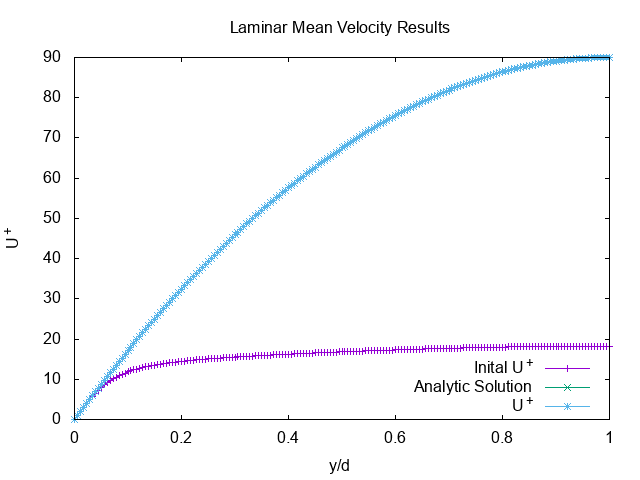
\includegraphics[width=.7\textwidth]{laminar}
 \caption{Laminar solution, Eqn. (\ref{eq:ssv2f1_nondim}), computed with
our $\overline{v^2}-f$ model. Note that our solution for $U$ sits on top of the
analytic solution.}
 \label{fig:laminar}
\end{figure}


%%% Re_tau = 180 case
Our next test was with $Re_\tau = 180$, which provided a more involved
verification of the model. Here we referred to $\overline{v^2} - f$ and DNS
solutions plotted in \cite{durbin180}. Plots from this paper are shown in Fig.
\ref{fig:durbin180} and we show steady solutions to each of the terms in
at this Reynolds number in Fig. \ref{fig:results_180}. Our solution looks almost
identical to Durbin's $\overline{v^2}-f$ results, and even disagrees with the DNS
data in the same regions of the channel. The model results agree with the DNS
data quite well, however, showing the strength of the $\overline{v^2}-f$ model
in capturing the near wall behavior in channel flow. Our verified results at
this stage gave us confidence that the model would behave well at high Reynolds
numbers.

\begin{figure}
 \centering
 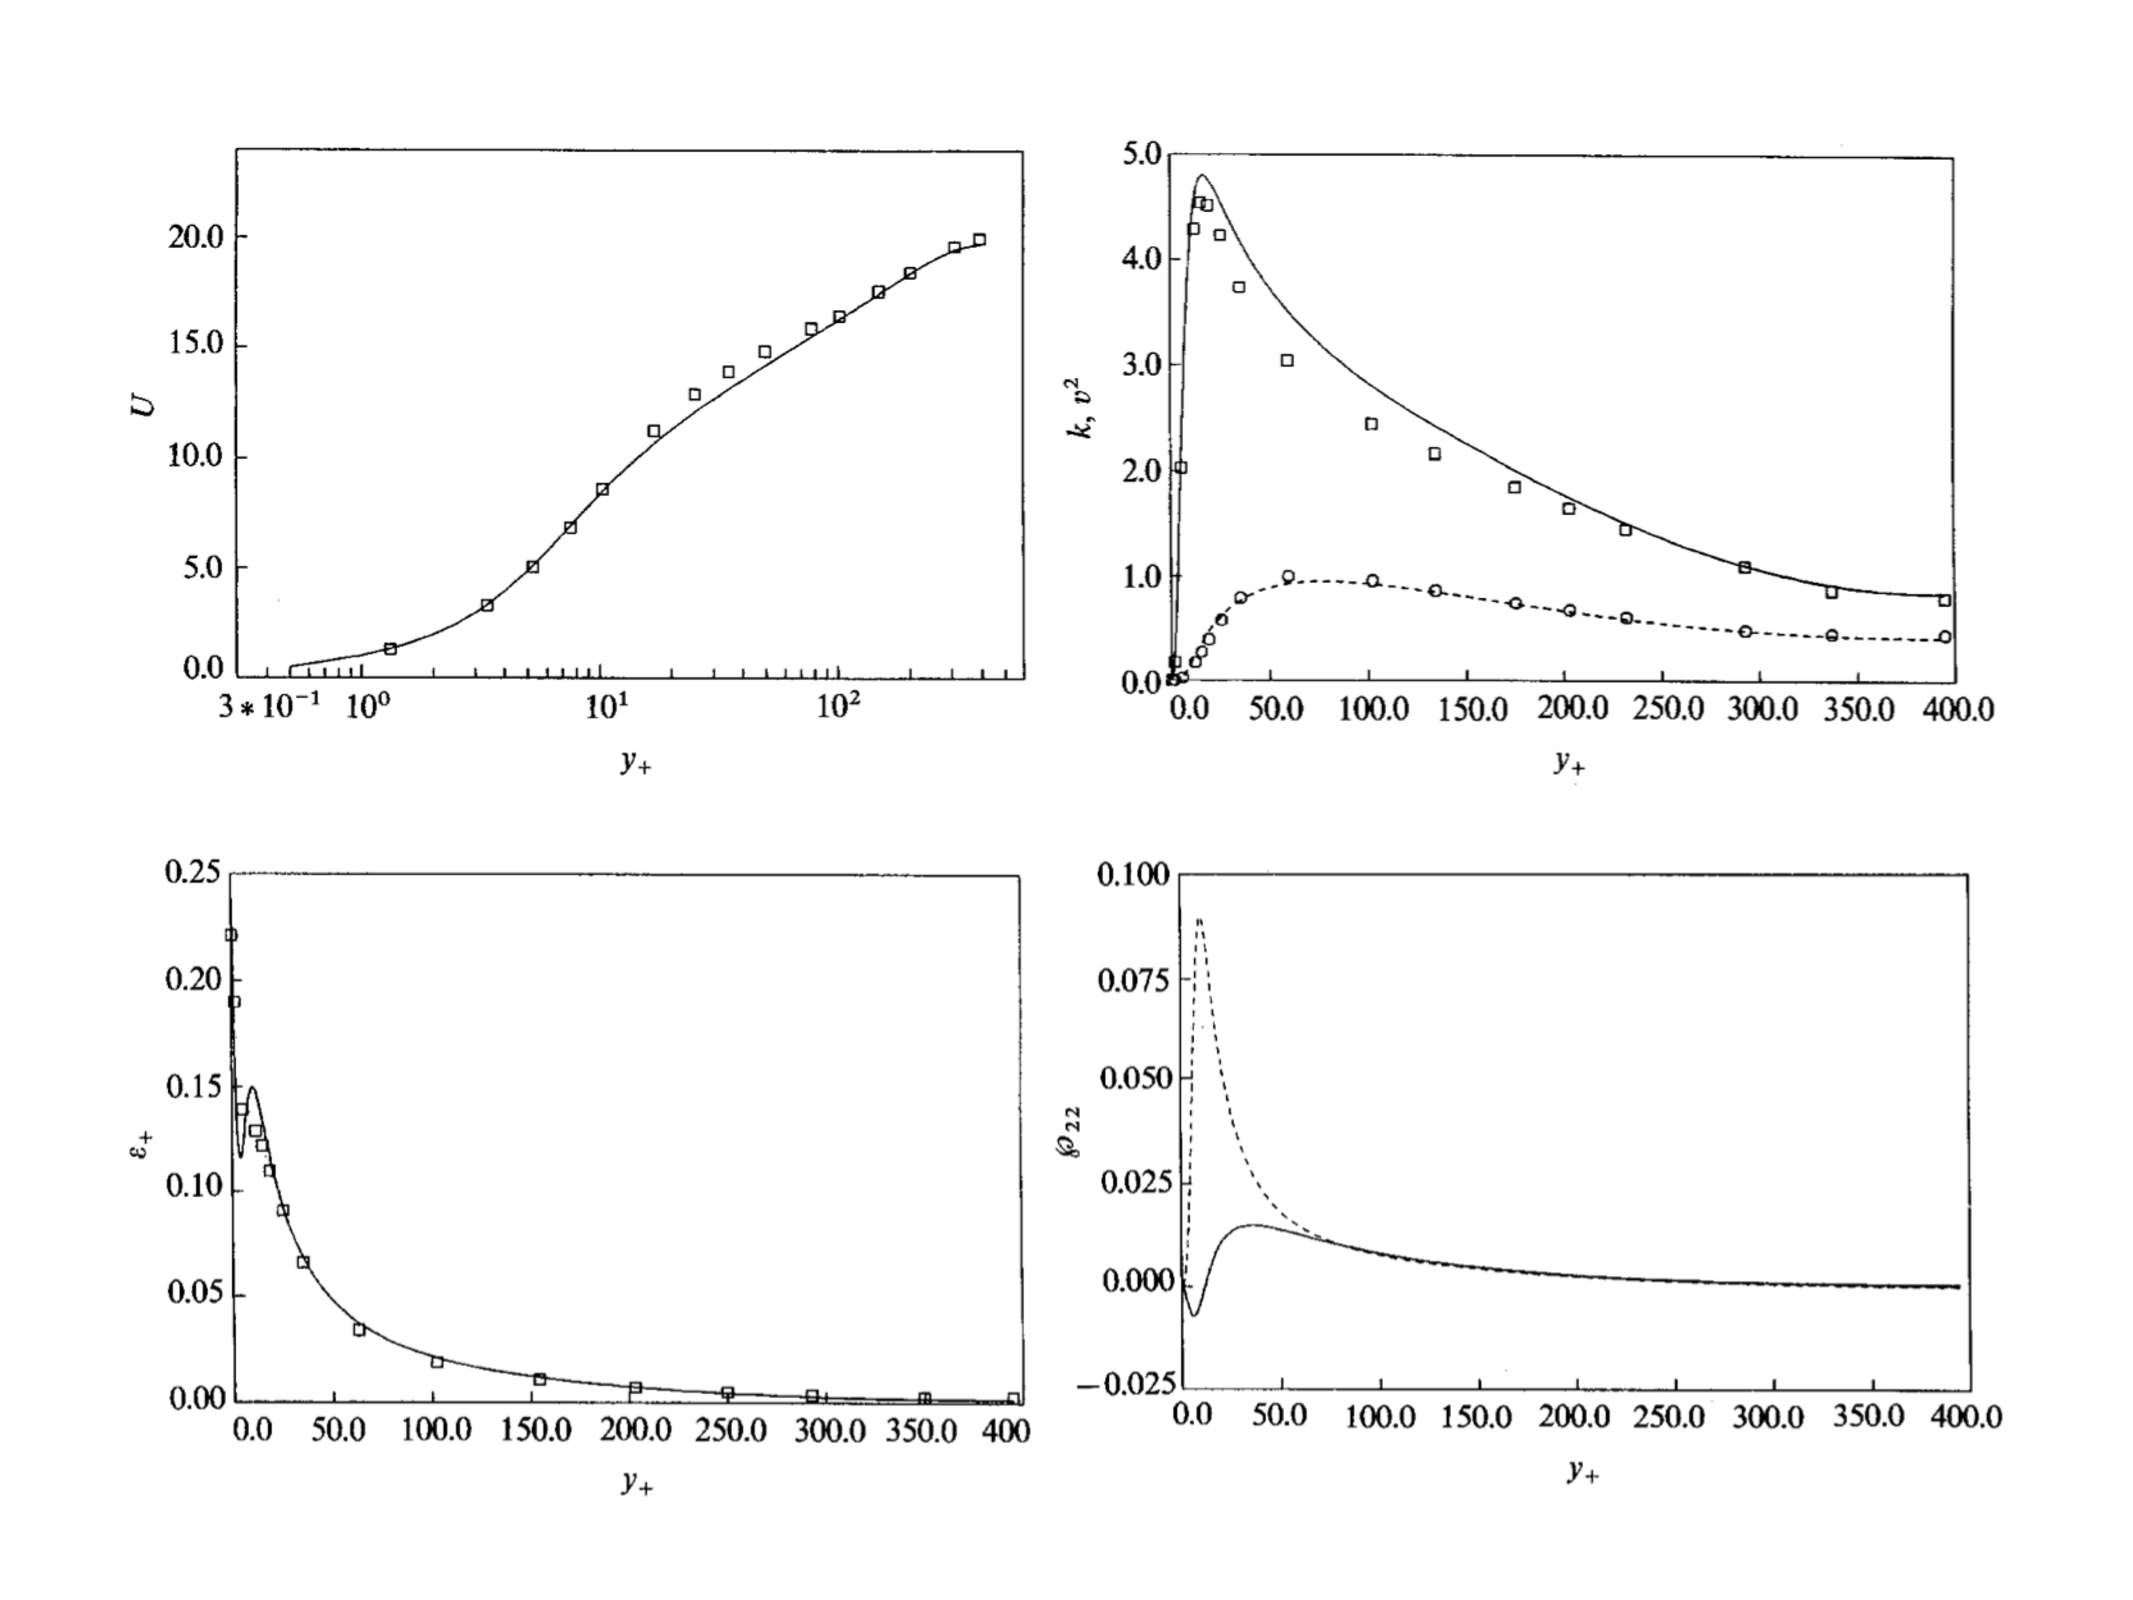
\includegraphics[width=\textwidth]{durbin180}
 \caption{Steady solutions for channel flow at $Re_\tau=180$ from DNS (circles)
and the $\overline{v^2}-f$ model (lines) taken from \cite{durbin180}. Each plot
is as labeled, and the solid black line on the bottom right figure shows $kf$.}
 \label{fig:durbin180}
\end{figure}

\begin{figure}
 \centering
 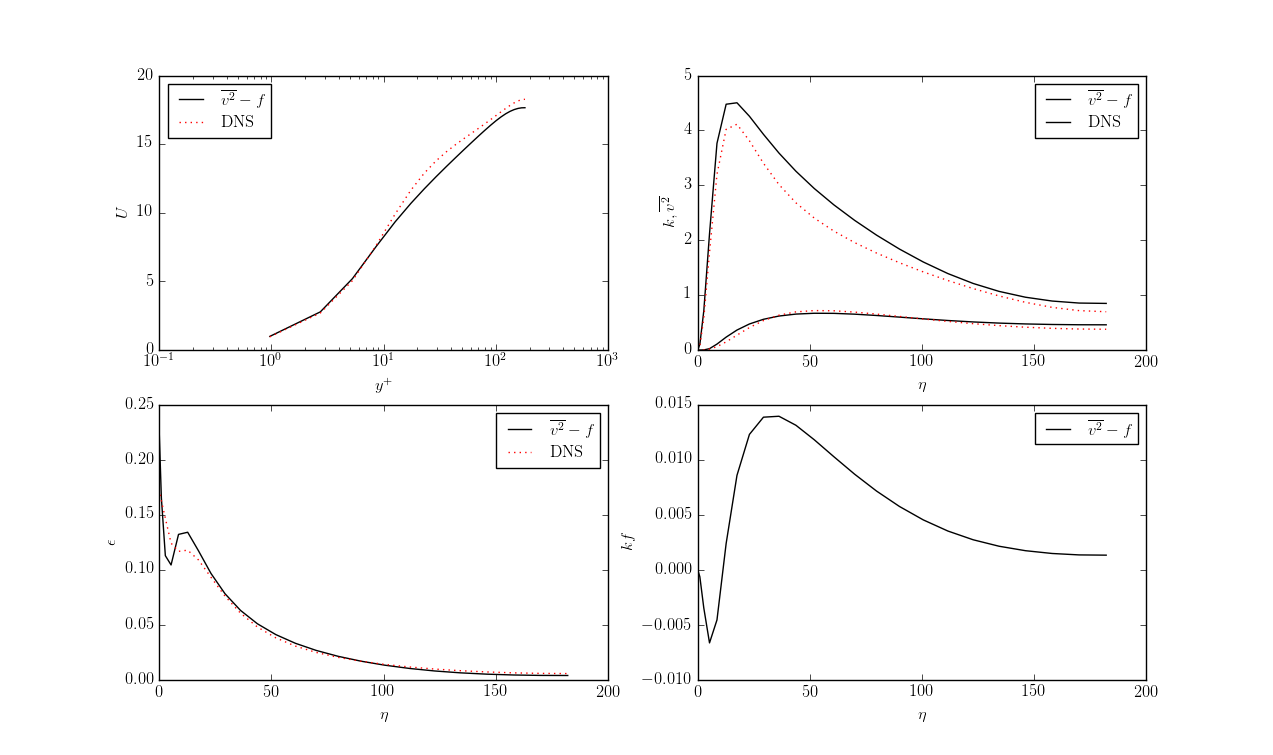
\includegraphics[width=\textwidth]{results_180}
 \caption{Steady state solution to the $\overline{v^2}-f$ model, Eqns.
(\ref{eq:ssv2f1_nondim})-(\ref{eq:ssv2f5_nondim}), at $Re_\tau=180$. The solid
black line shows results from our model, and the red dotted line shows
interpolated DNS results from \cite{Lee}. Note we show no initial data for $kf$
since $f$ is initialized at zero.}
 \label{fig:results_180}
\end{figure}


%%% Re_tau = 5200 case
After verifying our code on the $Re_{\tau} = 180$ case, we ran our code at $Re_{\tau} = 5200$, so as to compare it with the DNS results of \cite{Lee}. The results can be found......


\clearpage
\begin{thebibliography}{3}
\bibitem{Lee}
Lee, Myoungkyu and R.D. Moser, ``Direct numerical simulation of turbulent channel flow up to $\mathrm{Re}_{\tau}=5200$,'' J. Fluid Mech. 774 (2015) 395–415. doi:10.1017/jfm.2015.268.
\bibitem{Durbin}
    Durbin, Paul A., and BA Pettersson Reif. \textit{Statistical theory and
modeling for turbulent flows}. John Wiley \& Sons, 2011.
\bibitem{pope}
        Pope, Stephen B. \textit{Turbulent flows}. (2001): 2020.
\bibitem{durbin180}
        Durbin, Paul A. "Near-wall turbulence closure modeling without “damping
functions”." Theoretical and Computational Fluid Dynamics 3.1 (1991): 1-13.
 
\newpage



\end{thebibliography}


\end{document}
